\documentclass[sigconf,nonacm,10pt]{acmart}
\settopmatter{printacmref=false, printfolios=false}
\pagestyle{plain}
\usepackage{graphicx}
\usepackage{booktabs}
\usepackage{amsmath}
\usepackage{siunitx}
\emergencystretch=3em
\tolerance=1200
\hbadness=10000
\graphicspath{{../figs_mintfix_v2/}{../figs/}}

\newcommand{\SolEth}{SOL$\to$ETH}
\newcommand{\EthSol}{ETH$\to$SOL}
\newcommand{\Cexec}{C_{\text{exec}}}
\newcommand{\Pnet}{\Pi_{\text{net}}}

\title{Chapter 4 --- An End-to-End Empirical Study of Solana $\leftrightarrow$ Ethereum Cross-Chain Arbitrage}
\author{Anonymous}
\affiliation{\institution{-}\country{-}}

\begin{document}
\maketitle

% ══════════════════════════════════════════════════════════════════════════════
\section{Landscape of Solana $\leftrightarrow$ Ethereum Bridges}
\label{sec:bridges}
% ══════════════════════════════════════════════════════════════════════════════

Five general-purpose bridges currently support sustained asset transfers
between the Solana and Ethereum ecosystems: Wormhole Portal, LayerZero
V2, Mayan Finance, Relay, and Chainlink CCIP. They differ substantively
in trust model, fee schedule, and verification mechanism, resulting in
distinct latency, fee, and per-transfer-cap profiles.
Table~\ref{tab:bridges} summarises their main parameters alongside the
volume of bridge events we were able to collect for each.

\begin{table}[h]
  \centering
  \small
  \caption{Comparison of SOL~$\leftrightarrow$~ETH bridges}
  \label{tab:bridges}
  \begin{tabular}{lllr}
    \toprule
    \textbf{Protocol} & \textbf{Trust / Verification} & \textbf{Fee model} & \textbf{Records} \\
    \midrule
    Wormhole Portal   & Guardian-signed VAA        & Gas-based           & 42{,}181 \\
    LayerZero V2      & DVN verification           & DVN fees            & 271{,}813 \\
    Mayan Finance     & Dutch auction              & $\sim$3\,bps        & 10{,}653{,}600 \\
    Relay             & Intent-based fill          & Variable bps        & 107{,}220 \\
    Chainlink CCIP    & DON + risk manager         & LINK fees           & 2{,}115 \\
    \bottomrule
  \end{tabular}
\end{table}

Among these, Wormhole and CCIP adopt an attester-based ``messaging
layer $+$ token wrapping'' architecture; LayerZero is layered across
DVN attestation and Oracle/Relayer verification; Mayan and Relay
model cross-chain settlement as an ``intent/auction'' in which solvers
compete to fill orders. These architectural differences determine:
(i)~whether cross-chain events carry on-chain, 1:1-verifiable
cryptographic fingerprints; (ii)~whether each transfer can be paired
into an (src, dst) tuple through a single public field; and
(iii)~whether there is intermediary-priced latency--fee heterogeneity.
These three properties are exactly the preconditions for reconstructing
per-candidate arbitrage PnL in the remainder of the chapter.

% ══════════════════════════════════════════════════════════════════════════════
\section{Why Wormhole: Data and Candidate Construction}
\label{sec:data}
% ══════════════════════════════════════════════════════════════════════════════

\subsection{Why Wormhole Portal}

Of the five bridges above, we use Wormhole Portal as our sole
long-horizon sample source. Our reasoning is fourfold:
(i)~\emph{On-chain verifiability.} Portal Token Bridge transfers are
associated with Guardian-signed Verifiable Action Approvals (VAAs),
so that the Solana signature and Ethereum transaction hash of the
same transfer can be paired from on-chain and VAA evidence, without
relying on an off-chain trading ledger;
(ii)~\emph{Standardised pairing schema.} The Token Bridge contracts
on both chains use fixed emitter/recipient field layouts, so the
``actor'' primary key
$(arb_{\mathrm{sol}}, arb_{\mathrm{eth}})$ can be decoded directly
from on-chain data;
(iii)~\emph{Decoupled transport vs.\ execution.} Portal handles only
token wrap/unwrap; any subsequent DEX execution on the destination
chain is an independent on-chain event, allowing entry-swap,
bridge-leg, and exit-swap to be attributed separately;
(iv)~\emph{Broad token coverage.} Wormhole's WTT and NTT standards
cover many of the long-tail assets that appear in our candidate set.
This makes Portal a suitable setting for precise long-horizon
reconstruction, while still leaving cross-bridge selection effects
outside the scope of the present chapter.

\subsection{Data Collection Pipeline}
\label{sec:pipeline}

Figure~\ref{fig:pipeline} shows our five-stage collection and matching
pipeline. In our collection, the official Wormhole
\texttt{/operations} API was useful for recent VAA-indexed lookups but
was not sufficient as a complete year-long backfill source. We
therefore \emph{invert the pipeline} and start from the on-chain
Portal contracts on both legs:
(1)~on Ethereum and Solana, scan the Portal Token Bridge contract's
full log/instruction stream and parse the \texttt{src\_chain\_id} and
\texttt{dst\_chain\_id} of every bridge event;
(2)~for each event, use the Solana signature or Ethereum transaction
hash as a query key against Wormholescan's sig/hash search endpoint
to retrieve the corresponding VAA;
(3)~merge the two-chain signatures/hashes into a unified cross-chain
record keyed by the VAA identifier (\texttt{emitterChain} $+$
\texttt{sequence});
(4)~query Birdeye's \emph{1-second} price endpoint for the token-USD
rate at the entry and exit timestamps;
(5)~run a greedy attribution algorithm to assign same-wallet swaps
immediately before/after the bridge event to the candidate, yielding
tuples of the form
(direction, sol\_sig, eth\_hash, entry\_swaps, exit\_swaps,
$\Cexec^{\text{in}}, \Pnet$).

\begin{figure}[h]
  \centering
  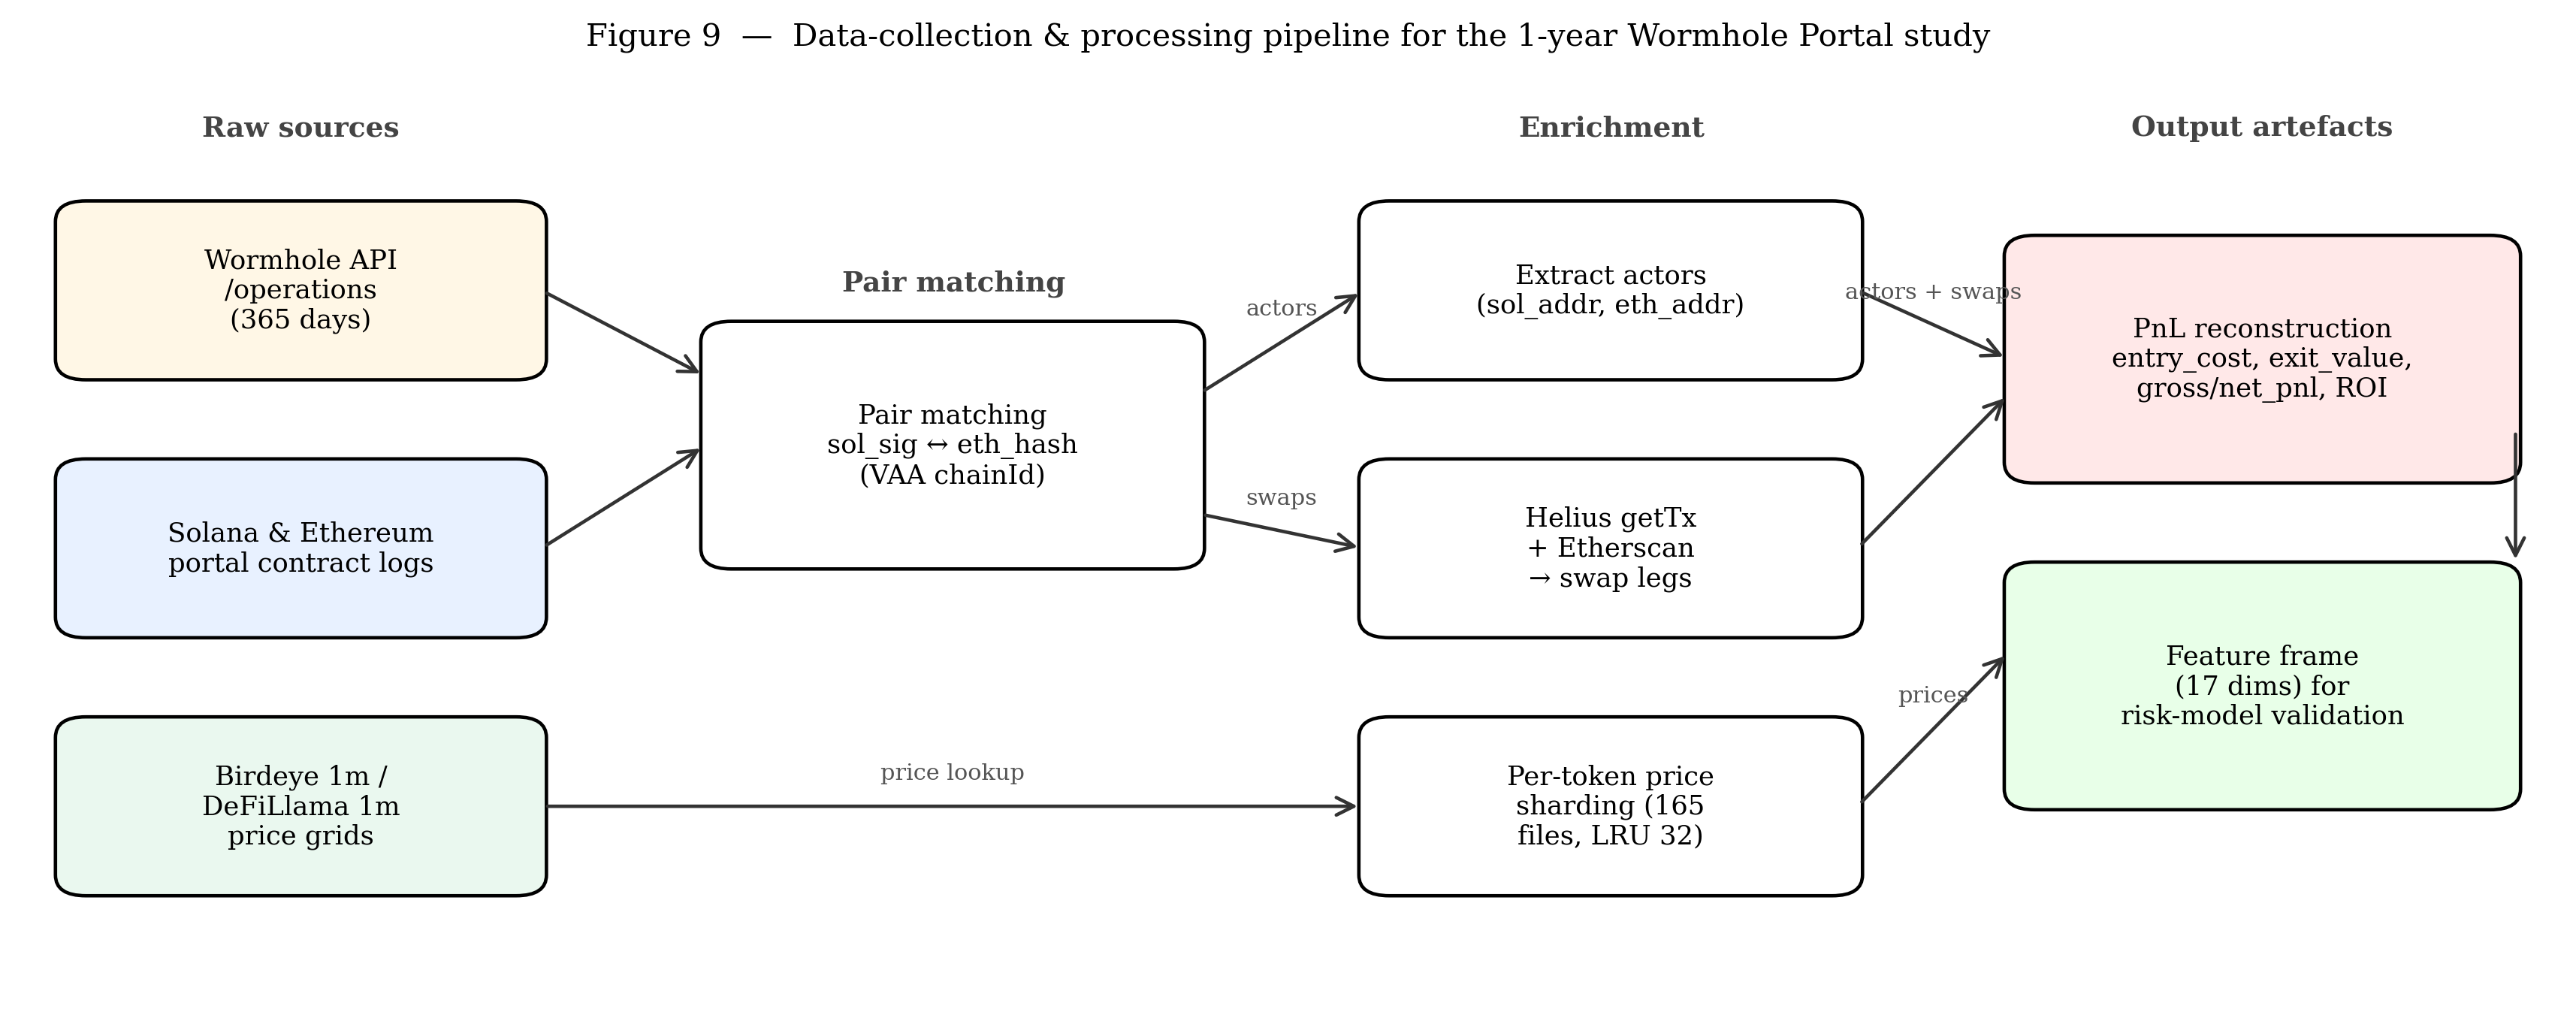
\includegraphics[width=\linewidth]{09_pipeline.png}
  \caption{Data collection and arbitrage-candidate construction pipeline.}
  \label{fig:pipeline}
\end{figure}

% ══════════════════════════════════════════════════════════════════════════════
\section{What drives cross-chain profit: descriptive evidence}
\label{sec:what-matters}
% ══════════════════════════════════════════════════════════════════════════════

This section answers the question: descriptively, which observables
are correlated with \emph{net PnL} $\Pnet$ and which are not?
Figure~\ref{fig:economics} reports six sub-results at the economic
level.

\begin{figure*}[t]
  \centering
  
\includegraphics[width=0.95\textwidth]{02_timing.png}
  \caption{Temporal structure of Wormhole Portal arbitrage:
  (a) bridge-latency CDF by direction;
  (b) swap--bridge time gap for entry and exit swaps;
  (c) ROI distribution stratified by bridge-latency tier.}
  \label{fig:timing}
\end{figure*}

\begin{figure*}[t]
  \centering
  
\includegraphics[width=0.95\textwidth]{03_economics.png}
  \caption{Economics of cross-chain arbitrage: (a) ROI histogram with
  inset CDF; (b) ROI CDF by direction; (c) log-scale distribution of
  entry capital and tier shading; (d) distribution of
  $\mathit{fee}/|\mathit{gross\ PnL}|$;
  (e) Gross vs.\ Net PnL scatter (colour-encoded by capital);
  (f) OLS regression of $\Pnet$ on $\log_{10}(\Cexec^{\text{in}})$.}
  \label{fig:economics}
\end{figure*}

\paragraph{Distribution shape (panels a/b).} ROI is heavy-tailed and
left-skewed, with median $+1.39\%$ and $78.0\%$ of samples positive;
the SOL~$\to$~ETH CDF has a slightly thinner left tail and
ETH~$\to$~SOL a slightly thicker one, but the two directional medians
differ by less than $1$ percentage point, so direction itself has
limited explanatory power. Table~\ref{tab:roi-quantiles} reports the
full quantile structure for reliable candidates. The heavy-tailed
profile is unambiguous: $p_{1}$ sits at $-49\%$ while $p_{99}$ reaches
$+152\%$; the ratio $\text{std}/|\text{median}|$ exceeds $48$; the
mean $+7.83\%$ is $5.6\times$ the median $+1.39\%$, dragged by a small
number of extreme positive samples.

\begin{table}[h]
  \centering
  \small
  \caption{ROI quantiles on reliable candidates ($n=29{,}340$, units \%)}
  \label{tab:roi-quantiles}
  \begin{tabular}{lr|lr|lr}
    \toprule
    \textbf{Stat.} & \textbf{Value} & \textbf{Quantile} & \textbf{Value} & \textbf{Quantile} & \textbf{Value} \\
    \midrule
    count & $29{,}340$    & $p_1$   & $-49.65$ & $p_{75}$ & $+3.77$ \\
    mean  & $+7.83$       & $p_5$   & $-4.15$  & $p_{90}$ & $+10.66$ \\
    std   & $67.07$       & $p_{10}$& $-1.51$  & $p_{95}$ & $+27.79$ \\
    min   & $-125.28$     & $p_{25}$& $+0.20$  & $p_{99}$ & $+152.40$ \\
    max   & $+5{,}204.09$ & $p_{50}$& $+1.39$  & ---      & --- \\
    \bottomrule
  \end{tabular}
\end{table}

The minimum ROI of $-125.28\%$ (loss exceeding $100\%$) is not a
calculation error: when $f_{\text{total}}>\Cexec^{\text{in}}$, the
ratio $\text{ROI}=\Pnet/\Cexec^{\text{in}}$ can mathematically cross
$-100\%$. The most extreme LOVE sample has entry $\$1.00$ and fees
$\$1.13$---a genuine economic loss, not a measurement artefact.

\paragraph{Capital is essentially unrelated to PnL (panels c/f).} On
a logarithmic x-axis, entry capital spans seven decades. Fitting an
OLS regression
\begin{equation}
  \Pnet = \alpha + \beta\cdot\log_{10}(\Cexec^{\text{in}}) + \varepsilon
  \label{eq:ols}
\end{equation}
on the $n=29{,}128$ reliable candidates yields
$\hat\beta=-1{,}085$~\$/decade with $R^2=0.0027$.
In words, \emph{entry capital explains only $0.27\%$ of the variance
in net PnL}. The binned-median curve in panel~(f) is approximately
flat and slightly positive over the $10^{2}$--$10^{4}$~USD band and
sinks at both ends---an inverted-U shape. This counter-intuitive
result refutes the folk assumption that cross-chain arbitrage is a
linearly capital-scalable business.

\paragraph{Fees are a first-order constraint (panels d/e).} The
fee-rate distribution is extremely wide; the median
$\mathit{fee}/|\mathit{gross}|=0.053$, but $2.8\%$ of candidates
suffer $\mathit{fee}>|\mathit{gross}|$---severe fee erosion. In
panel~(e) every point lies strictly below the $y=x$ line; the
vertical displacement visualises the fee cost directly, and the dense
lower-left cluster corresponds to the many small-volume losses whose
gross margin failed to cover gas.

\paragraph{Temporal structure (Fig.~\ref{fig:timing}).}
Figure~\ref{fig:timing} characterises the time-side properties of
cross-chain candidates from three angles:
(a) bridge-latency CDF by direction---SOL$\to$ETH (blue) has
median $\sim\!34$~s while ETH$\to$SOL (red) has median
$\sim\!1{,}011$~s ($\sim\!17$~min), a $\sim\!30\times$ asymmetry
that matches the gap between Solana's sub-second slot finality and
Ethereum's two-epoch finality window; the two CDFs converge only in
the far right tail (both $p_{99}\!>\!4{,}000$~s);
(b) swap-to-bridge time gap---the entry-side gap has a median
$\sim\!12$~s while the exit-side is longer ($\sim\!24$~s), with a
right tail extending into the hour range (a small number of
candidates hold the bridged position before exit), which justifies
attributing pre/post bridge swaps of the same wallet to the same
cross-chain arbitrage candidate;
(c) ROI boxplot by latency tier---medians are non-monotone across
short and medium horizons: $<\!60$~s ($n=14{,}599$, median
$+1.39\%$), $60$--$300$~s ($n=2{,}639$, median $+1.04\%$), and
$300$~s--$1$~h ($n=14{,}449$, median $+1.50\%$) are broadly
comparable, while the $1$--$24$~h tier collapses to $+0.13\%$ and
the $>\!24$~h tier to $-1.35\%$. Panel~(c) therefore suggests that
very long holding delays are associated with weaker outcomes, rather
than a strictly monotone latency--ROI relation at all horizons.

\paragraph{Summary of ``what matters / what does not.''}
Table~\ref{tab:univar} collects the descriptive evidence above. These
are all \emph{univariate} claims; some of the variables are
re-evaluated under the multivariate model in
Section~\ref{sec:model}.

\begin{table}[h]
  \centering
  \small
  \caption{Descriptive relations between $\Pnet$ and each variable}
  \label{tab:univar}
  \begin{tabular}{lll}
    \toprule
    \textbf{Variable} & \textbf{Relation} & \textbf{Evidence} \\
    \midrule
    Entry spread     & Positive, significant     & Prior work + tiering \\
    Bridge latency   & Negative, significant     & Fig.~\ref{fig:timing}(c) + model \\
    Liquidity depth  & Non-linear                & Liquidity-tier strata \\
    Fees             & Negative (identity)       & Fig.~\ref{fig:economics}(d/e) \\
    Entry capital    & $R^2\!=\!0.003$, near-null & Fig.~\ref{fig:economics}(f) \\
    Direction        & Gap $<\!1$\,pp             & Fig.~\ref{fig:economics}(b) \\
    Hour of day      & Approximately uniform     & (omitted) \\
    Swap split count & No significant effect     & Fig.~\ref{fig:timing}(b) \\
    \bottomrule
  \end{tabular}
\end{table}

% ══════════════════════════════════════════════════════════════════════════════
\section{Integrated Modelling and Experiments}
\label{sec:model}
% ══════════════════════════════════════════════════════════════════════════════

The conclusions in \S\ref{sec:what-matters} are all univariate. If the
features interact, univariate relations can mislead. This section
reassesses both the direction and magnitude of $\Pnet$ via a
multivariate non-linear model under two parallel targets:
a \emph{regression} predicting the dollar amount of $\Pnet$, and a
\emph{classification} predicting $\mathbf{1}\{\Pnet>0\}$.

\subsection{Feature set}
\label{sec:features}

We assemble $17$ features covering six hypothesised driver families,
all observable at the candidate level:
\emph{direction / time} (\texttt{dir\_sol\_to\_eth}, \texttt{hour\_utc});
\emph{size / latency} (\texttt{log\_size}, \texttt{log\_latency});
\emph{atomicity} (\texttt{atomic\_entry\_same\_block},
\texttt{atomic\_exit\_same\_block});
\emph{swap--bridge timing} (\texttt{entry\_delta\_bridge\_sec},
\texttt{exit\_delta\_bridge\_sec},
\texttt{n\_entry\_swaps}, \texttt{n\_exit\_swaps});
\emph{measurement completeness} (\texttt{entry\_coverage},
\texttt{exit\_coverage});
\emph{liquidity tiers and market} (\texttt{liq\_dead},
\texttt{liq\_thin}, \texttt{liq\_healthy}, \texttt{entry\_gap\_pct},
\texttt{actor\_trade\_count}).

\subsection{Model specification}

Both models share the same additive tree ensemble:
\begin{equation}
F_M(x) \;=\; \sum_{m=1}^{M} \eta \cdot h_m(x),
\label{eq:gbm}
\end{equation}
where $h_m$ is a depth-$3$ regression tree, $M=200$, and
$\eta=0.05$. Each tree fits the negative functional gradient of the
current loss:
\begin{equation}
h_m \;=\; \arg\min_{h}\,\sum_{i=1}^{n}
L\!\bigl(y_i,\; F_{m-1}(x_i)+h(x_i)\bigr),
\label{eq:gbm-update}
\end{equation}
with $\text{subsample}=0.8$ applied per tree to reduce variance.

\paragraph{Regression target (``how much'').}
The target is a USD-winsorised $\Pnet$:
\begin{equation}
y^{\text{reg}}_i \;=\; \operatorname{clip}\!\bigl(\Pi_{\text{net},i},\;
-\$100,\; +\$500\bigr),
\label{eq:reg-target}
\end{equation}
with squared-error loss
$L_{\text{reg}}(y,\hat y)=\tfrac12(y-\hat y)^2$.
The bounds $[-\$100,+\$500]$ are chosen for four reasons:
(i)~the raw $\Pnet$ distribution is extremely heavy-tailed
($\min\!\approx\!-\$2.07\text{M}$, $\max\!\approx\!+\$428\text{K}$),
so without clipping a single outlier contributes $\mathcal{O}(10^{12})$
gradient under MSE and dominates the fit;
(ii)~$[-\$100,+\$500]$ contains $95.8\%$ of candidates
(only $2.5\%$ below, $1.7\%$ above), i.e.\ almost all samples keep
their original values and only the tails are winsorised;
(iii)~the bounds are deliberately asymmetric because the distribution
itself is right-skewed with median $+\$3.14$ and p75~$\approx+\$10$,
while the losing tail concentrates around the per-trade fee scale
($\sim\!\$20$--$50$), so $-\$100$ already corresponds to
``clearly bad'' and $+\$500$ preserves the heterogeneity of winners
up to the top $\sim\!3\%$;
(iv)~the clip applies only to the regression head; the classification
target $y^{\text{cls}}$ still sees raw signs, so no information about
large losses or large gains is lost at the system level.

\paragraph{Classification target (``whether profitable'').}
The target is a profit indicator:
\begin{equation}
y^{\text{cls}}_i \;=\; \mathbf{1}\{\Pi_{\text{net},i}>0\},
\label{eq:cls-target}
\end{equation}
with binary cross-entropy
$L_{\text{cls}}(y,\hat p)=-y\log\hat p-(1-y)\log(1-\hat p)$,
producing a probability
$\hat p_i=\sigma\!\bigl(F_M(x_i)\bigr)$. A trading decision is
obtained via a threshold $\tau$:
$\hat y^{\text{cls}}_i=\mathbf{1}\{\hat p_i>\tau\}$.

\subsection{Evaluation protocol}

The training set is restricted to candidates with
\texttt{pnl\_complete} and no missing features, giving $n=15{,}497$.
We use $K=5$-fold shuffled KFold (\texttt{random\_state}$=42$):
each fold trains on $4/5$ of the data and tests on the held-out
$1/5$. Cross-validated scores are averaged across folds:
\begin{equation}
R^2_{\text{CV}} = \tfrac{1}{K}\sum_{k=1}^{K} R^2_k,\quad
\text{AUC}_{\text{CV}} = \tfrac{1}{K}\sum_{k=1}^{K} \text{AUC}_k.
\label{eq:cv}
\end{equation}
Regression reports $R^2$, MAE, Median AE; classification reports
AUC, log-loss, and at two operating thresholds
$\tau\in\{0.5,\,0.8\}$,
\begin{equation}
\text{Precision}=\tfrac{TP}{TP+FP},\quad
\text{Recall}=\tfrac{TP}{TP+FN}.
\label{eq:pr}
\end{equation}
The naive classification baseline is ``always predict profit,''
whose accuracy equals the positive rate
$\bar y^{\text{cls}}=73.85\%$.
Because the split is shuffled at the candidate level, these scores
measure within-sample predictive structure rather than deployment
performance for a new bot, actor, or market regime. Actor-held-out
and time-forward validation are therefore treated as robustness checks
outside the scope of this chapter.

\subsection{Cross-validated results}

Table~\ref{tab:model} summarises 5-fold CV performance. The regressor
reaches $R^2_{\text{CV}}=0.799\pm 0.027$---more than two orders of
magnitude above Eq.~\eqref{eq:ols}'s univariate $R^2=0.003$,
indicating that \emph{$\Pnet$ has strong within-sample predictive
structure given the $17$-feature set, but only under a multivariate
non-linear model}. Median AE $=\$5.13$
implies at least half of the samples are predicted within $\pm\$5$;
the gap between MAE $=\$17.14$ and Median AE (a factor of $3.3$)
indicates a fat-tailed error distribution---a minority of extreme
samples remain under-fit, confirming the need for the clipping in
Eq.~\eqref{eq:reg-target}.

The classifier's AUC is $0.866\pm 0.005$: substantially above
the $0.5$ random baseline but well below the $1.0$ perfectly-separable
limit---reflecting intrinsic randomness in cross-chain arbitrage
(counterparty flow, Guardian-signing jitter) that the present feature
set cannot exhaust. At $\tau=0.5$, accuracy is $82.3\%$, $+8.5$~pp
over the naive $\bar y^{\text{cls}}=73.85\%$ baseline. Raising
$\tau$ to $0.8$ trades recall for precision: precision rises to
$93.5\%$ while recall falls to $66.2\%$---within this shuffled-CV
evaluation, retaining only predictions with $\hat p_i>0.8$ produces a
high-precision subset at the cost of missing $34\%$ of profitable
cases. This precision--recall schedule suggests that the classifier
can rank candidates by ex-post profitability risk, but it should not
be interpreted as a validated live trading rule without actor-held-out
or time-forward testing. Log-loss $=0.386$ is also below the binomial
baseline of $0.576$.

\begin{table}[h]
  \centering
  \small
  \caption{Model performance (5-fold CV, $n=15{,}497$)}
  \label{tab:model}
  \begin{tabular}{ll}
    \toprule
    \textbf{Metric} & \textbf{Value} \\
    \midrule
    Regressor $R^2_{\text{CV}}$              & $0.7987 \pm 0.0269$ \\
    Regressor MAE                            & \$17.14 \\
    Regressor Median AE                      & \$5.13 \\
    Classifier AUC$_{\text{CV}}$             & $0.8658 \pm 0.0052$ \\
    Classifier accuracy at $\tau=0.5$        & $82.3\%$ (baseline $73.9\%$) \\
    Classifier precision at $\tau=0.8$       & $93.5\%$ (recall $66.2\%$) \\
    Classifier log-loss                      & $0.3864$ \\
    \bottomrule
  \end{tabular}
\end{table}

% ══════════════════════════════════════════════════════════════════════════════
\section{Limitations}
\label{sec:limitations}
% ══════════════════════════════════════════════════════════════════════════════

\paragraph{Sensitivity to the dust-filter threshold.} We set the
dust-filter threshold at $\Cexec^{\text{in}}<\$1$, motivated by the
\$1--\$5 physical floor of Ethereum L1 swap gas. Raising the
threshold to \$5 increases the set of excluded rows from $12$ to
$116$ ($\sim 0.4\%$), lowers the ROI mean on the reliable
subset from $+7.83\%$ to $+6.88\%$, while leaving the median
essentially unchanged ($+1.39\%\!\to\!+1.38\%$). The GBM results of
Section~\ref{sec:model} ($R^2$, AUC, Median AE) do not
change materially under either threshold. We keep the more
conservative \$1 threshold to maximise sample size and avoid
discarding legitimate small-size trades where ``fees exceed
entry'' is a real economic loss.

\paragraph{Single-bridge sample bias.} We collect candidates only
from Wormhole Portal, leaving LayerZero~V2, Mayan, Relay, and CCIP
out of scope.
Section~\ref{sec:bridges} argued that Wormhole provides broad
long-tail token coverage and a pairing structure that permits
candidate-level PnL reconstruction. That said, Portal's end-to-end
latency is a median of $\sim\!13$~s (Solana finality) plus
$\sim\!13$~min (two Ethereum epochs)---numbers specific to Wormhole.
On LayerZero or intent-based Mayan/Relay, the latency mechanism, tail
shape, solver behaviour, and arbitrage window differ substantially,
so the chapter's model coefficients and $R^2_{\text{CV}}$ should not
be extrapolated to other bridges; a rigorous cross-bridge comparison
is future work.

\paragraph{Observation window and regime shifts.} The dataset spans
approximately $365$ days, over which Solana/Ethereum fee regimes,
Wormhole's Guardian signing cadence, and the behaviour of top bots
may all have undergone regime shifts. The model in this chapter is
a \emph{mixed-period} average and is not segmented; splitting the
window into distinct regimes may cause both model coefficients and
CV scores to drift. Regime identification and segment-wise modelling
are left to future work.

\end{document}
